\section{Python Overview}
\begin{itemize}
    \item \textbf{Ursprung:} Entwickelt von Guido van Rossum mit Fokus auf Einfachheit und Stärke.
    \item \textbf{Standardbib.:} Bekannt für "Batteries included", also eine umfangreiche, integrierte Bibliothek.
    \item \textbf{Ökosystem:} Für Ingenieure ersetzt Python Matlab-Toolboxen durch Pakete wie \textbf{NumPy} (Zahlen), \textbf{pandas} (Daten) und \textbf{matplotlib} (Grafik).
\end{itemize}

\section{Variablen und Objekte}
In Python ist alles ein Objekt. Variablen sind keine Container, sondern an Objekte gebundene \textbf{Referenzen} (Pointer).

\begin{minipage}{0.4\columnwidth}
    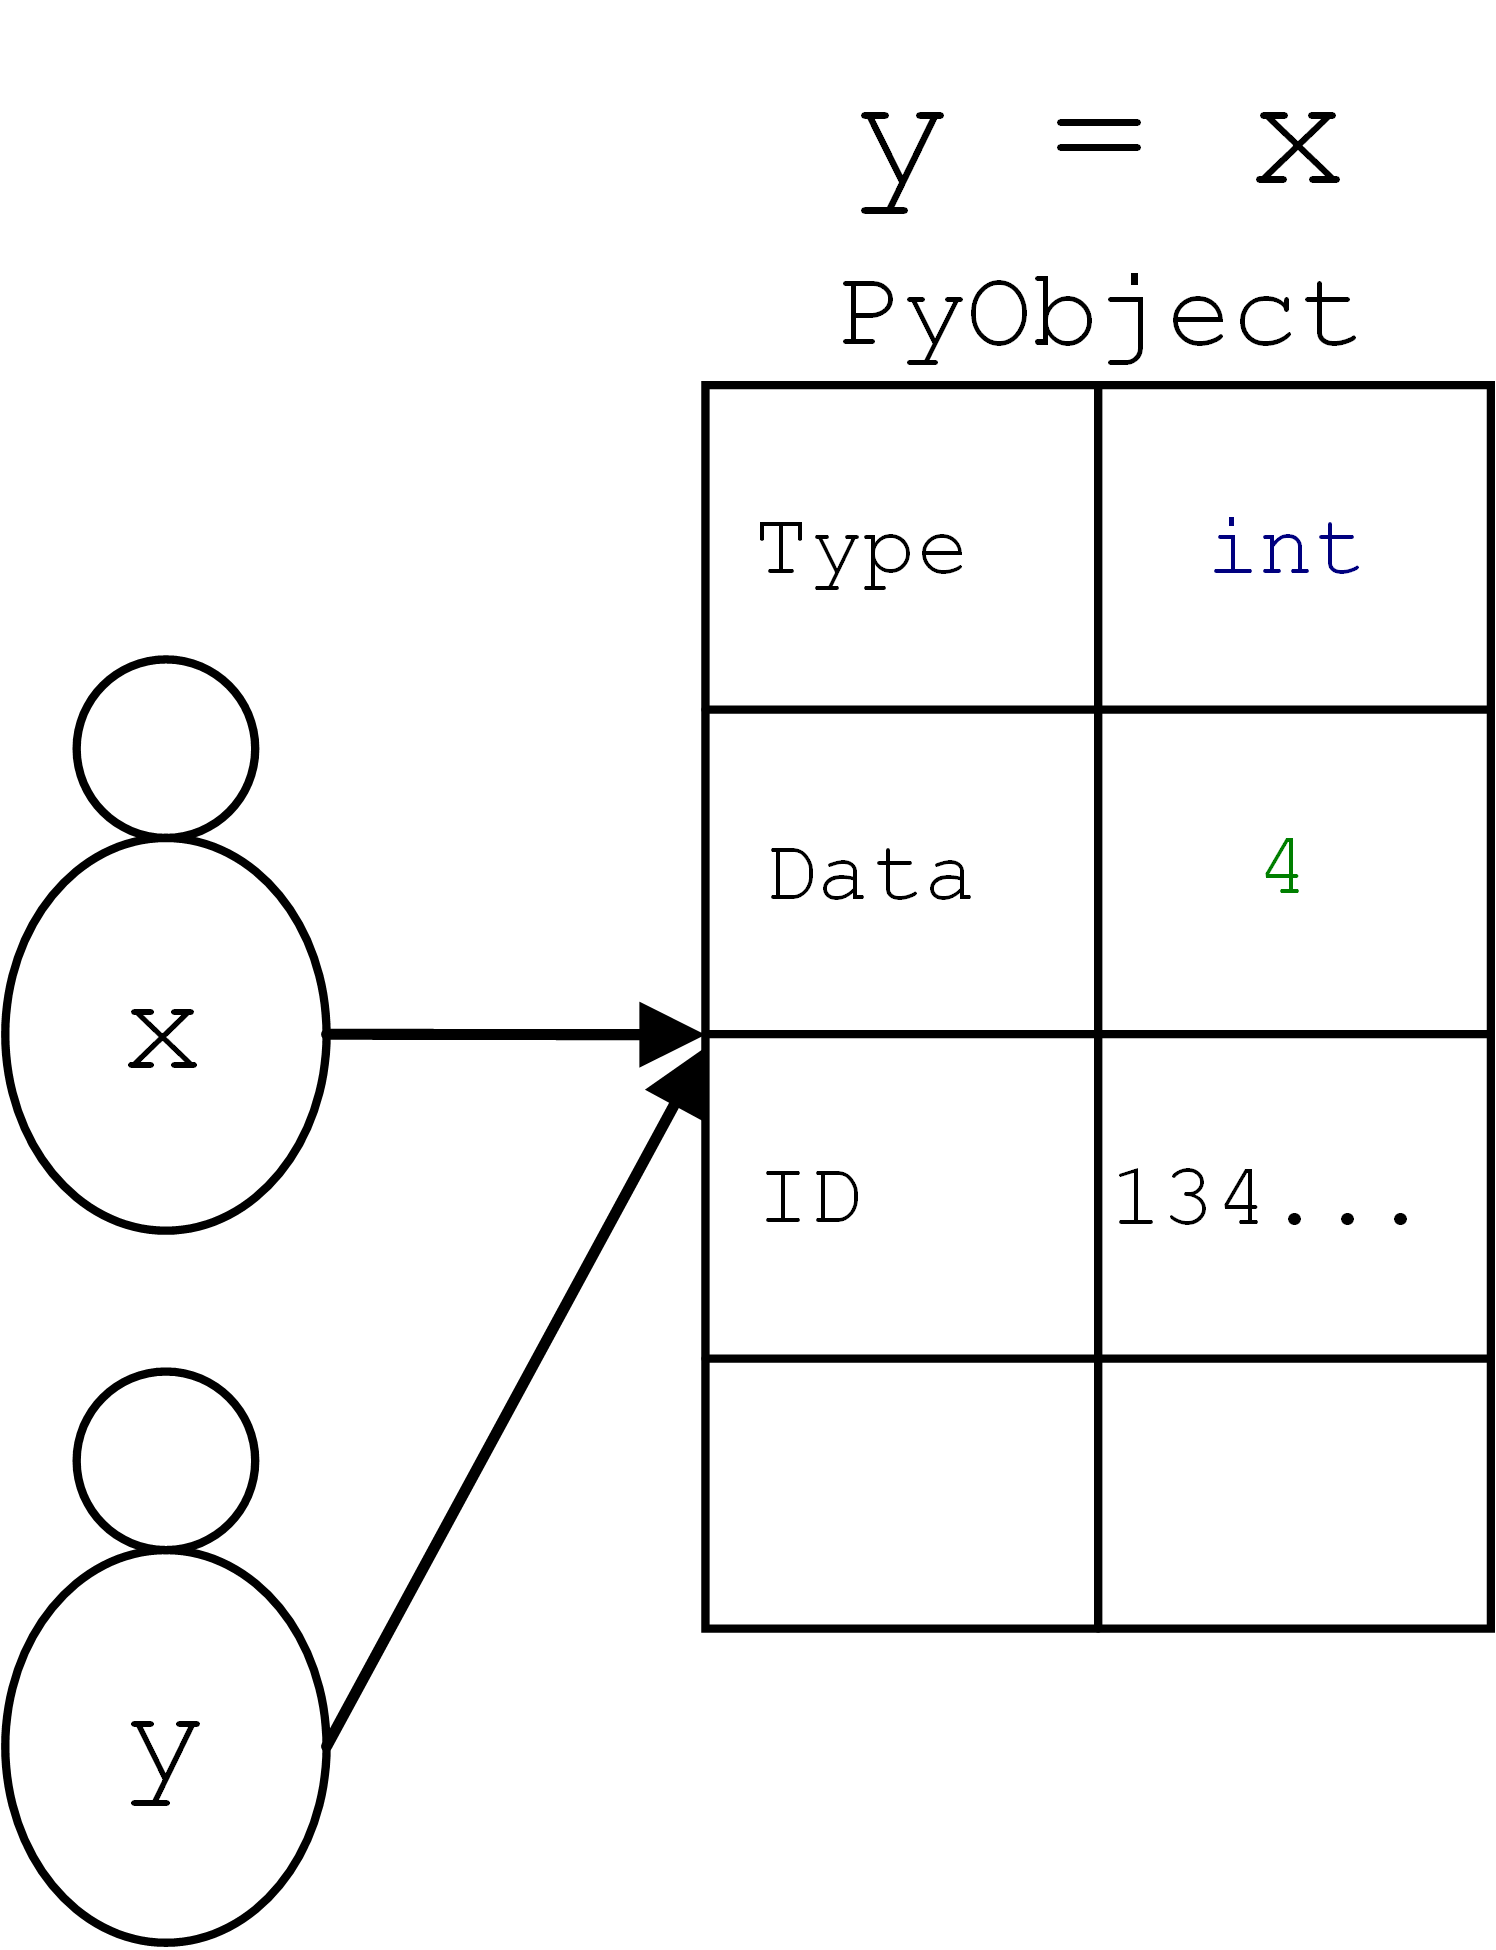
\includegraphics[width=\linewidth]{images/var_2.png}
\end{minipage}\hfil
\begin{minipage}{0.4\columnwidth}
    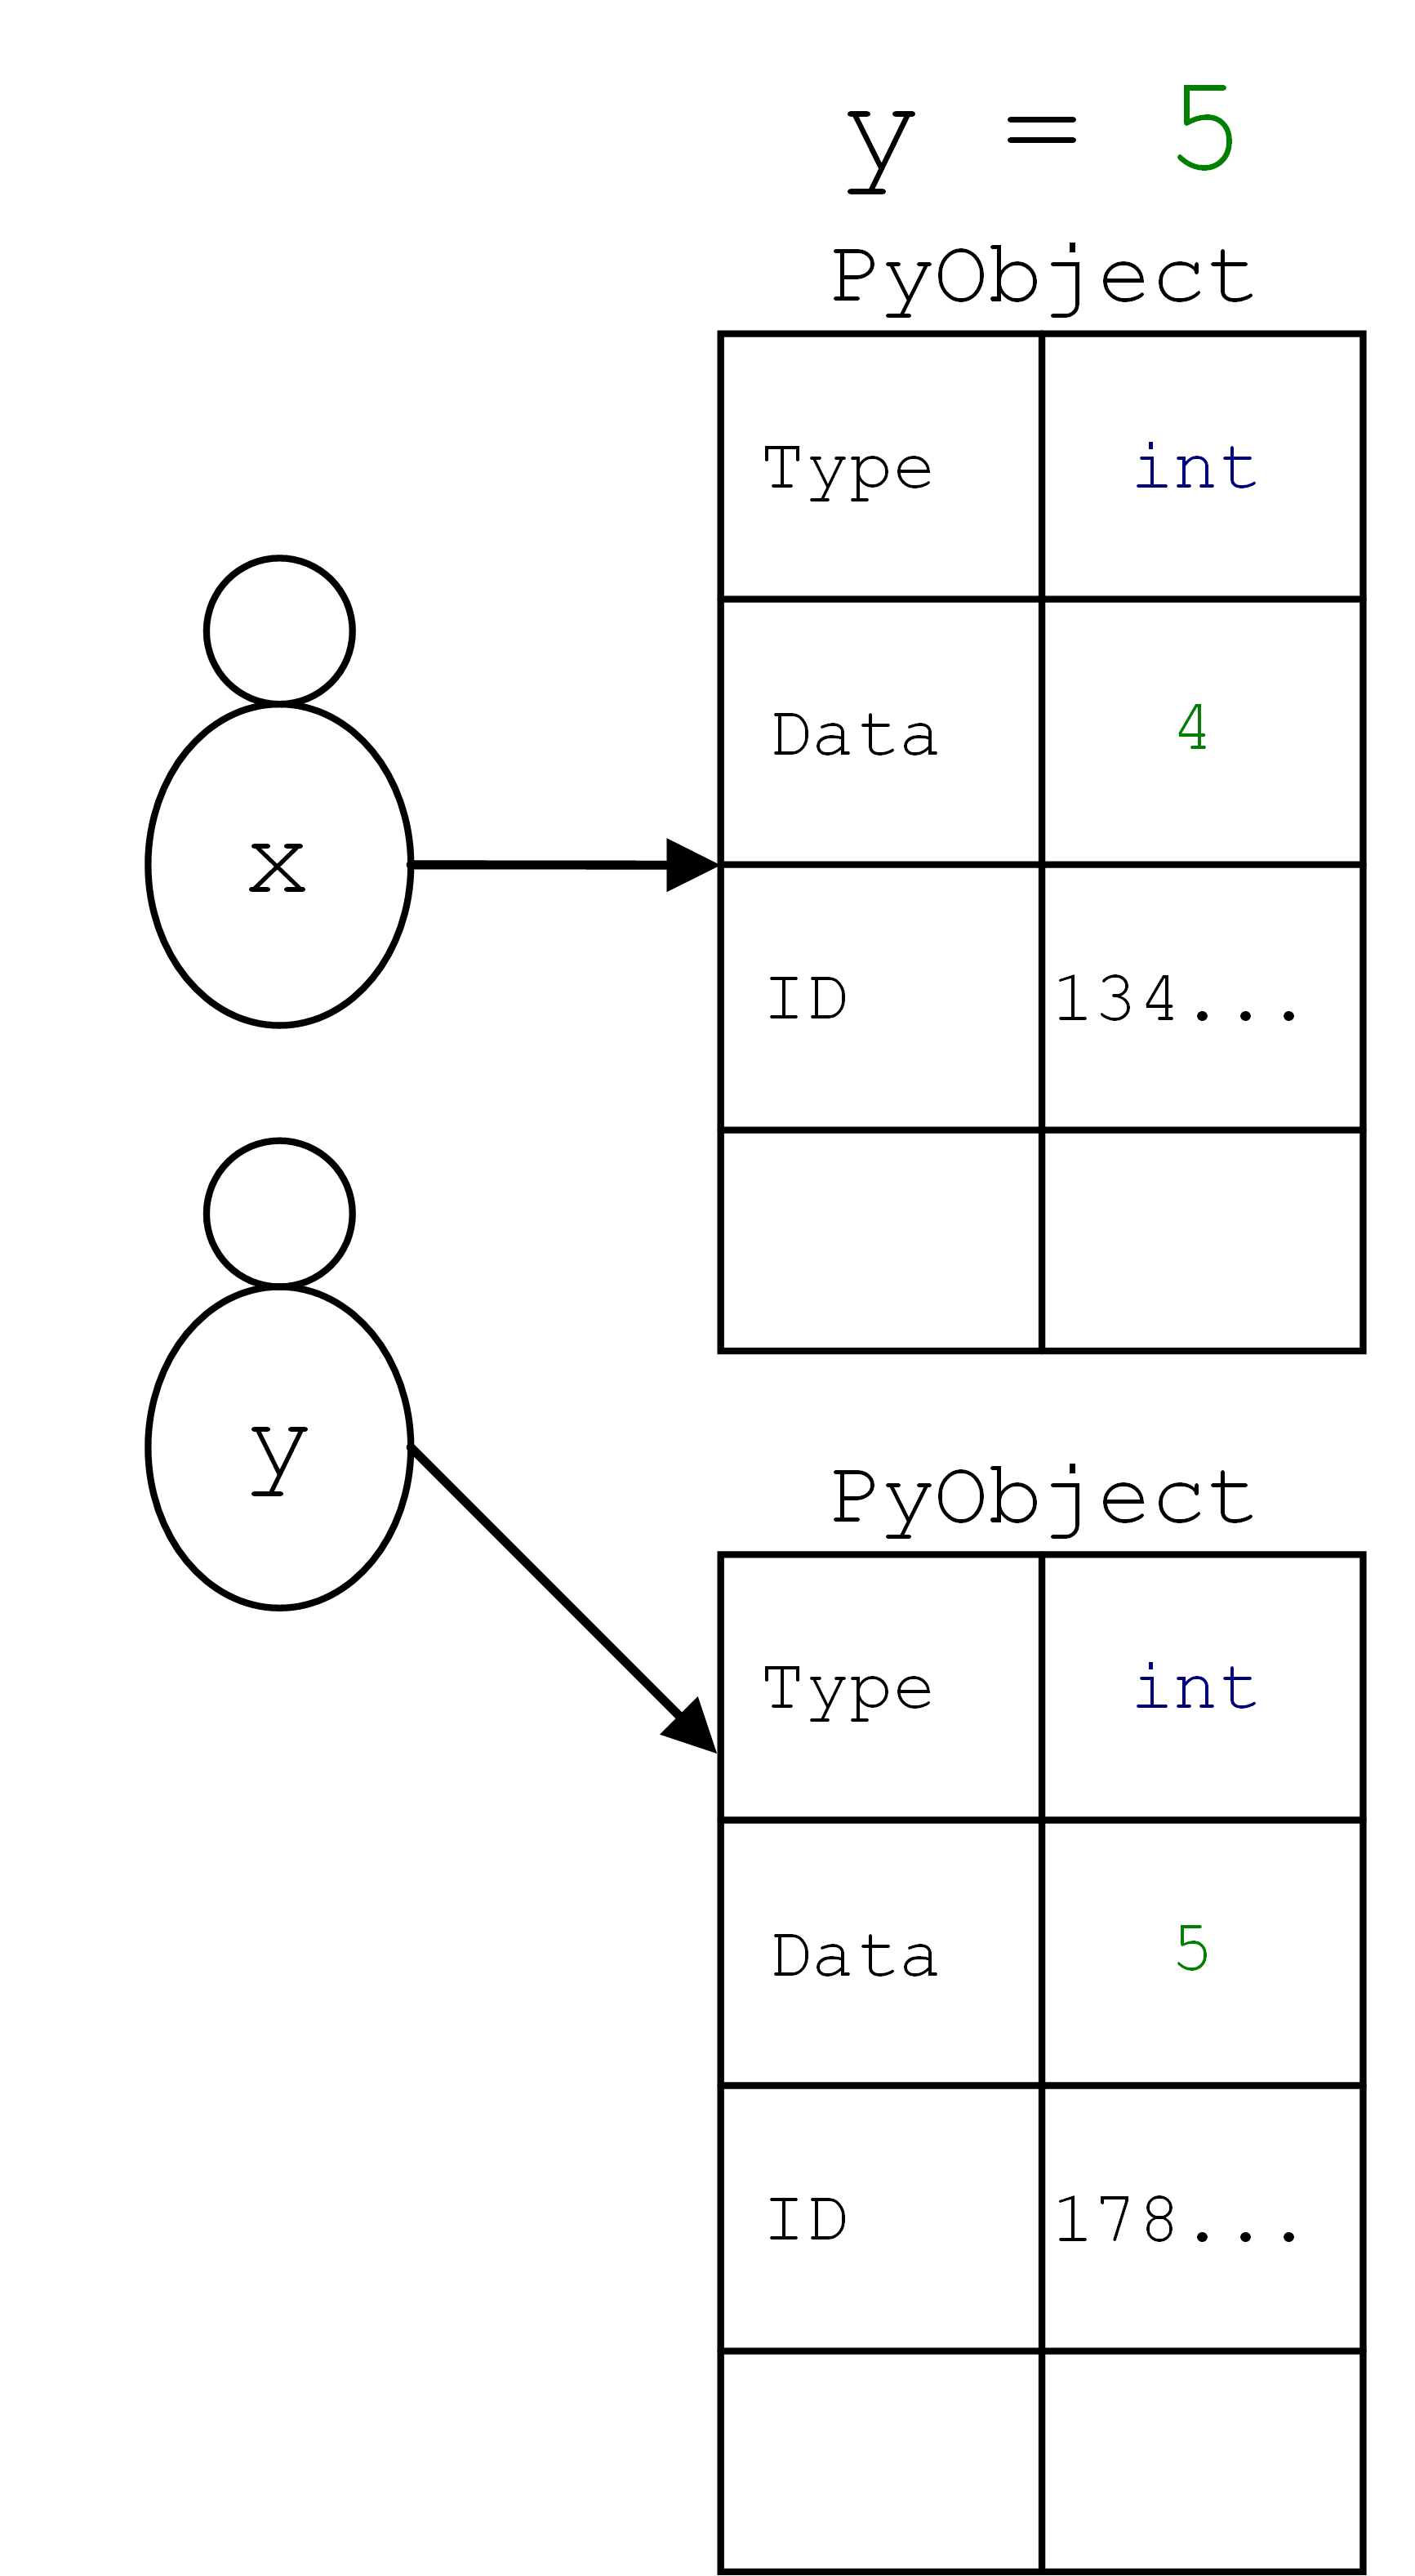
\includegraphics[width=\linewidth]{images/var_3.png}
\end{minipage}

\subsection{Integrierte Datentypen}
\begin{center}
    \begin{tabular}{llll}
        \toprule
        \textbf{Kategorie} & \textbf{Datentyp} & \textbf{Veränderbarkeit} & \textbf{Falsch-Wert} \\ \midrule
        \textbf{None} & \texttt{NoneType} & Unveränderlich & \texttt{None} \\ \addlinespace
        \textbf{Numerisch} & \texttt{int} & Unveränderlich & \texttt{0} \\
        & \texttt{float} & Unveränderlich & \texttt{0.0} \\
        & \texttt{bool} & Unveränderlich & \texttt{False} \\
        & \texttt{complex} & Unveränderlich & \texttt{0 + 0j} \\ \addlinespace
        \textbf{Sequenz} & \texttt{str} & Unveränderlich & \texttt{''} \\
        & \texttt{list} & Veränderlich & \texttt{[]} \\
        & \texttt{tuple} & Unveränderlich & \texttt{()} \\
        & \texttt{bytes} & Unveränderlich & \texttt{b''} \\
        & \texttt{bytearray} & Veränderlich & \texttt{bytearray(b'')} \\ \addlinespace
        \textbf{Mengen} & \texttt{set} & Veränderlich & \texttt{set()} \\
        & \texttt{frozenset} & Unveränderlich & \texttt{frozenset()} \\ \addlinespace
        \textbf{Assoziativ} & \texttt{dict} & Veränderlich & \texttt{\{\}} \\ \bottomrule
    \end{tabular}
\end{center}

\subsection{Veränderbarkeit}
\begin{itemize}
    \item \textbf{Unveränderlich:} Objekte, die nach Erstellung nicht modifiziert werden können (z.B. \texttt{int}, \texttt{float}, \texttt{str}, \texttt{tuple}). Wertänderung erzeugt real ein komplett neues Objekt im Speicher.
    \item \textbf{Veränderlich:} Objekte, die direkt in-place modifiziert werden können (z.B. \texttt{list}, \texttt{set}, \texttt{dict}).
\end{itemize}\vspace{1em}
Die Speicheradresse eines Objekts kann mit der Funktion \texttt{id()} visualisiert werden. 

Sie gibt eine eindeutige Ganzzahl für das jeweilige Objekt zurück.

\section{Namensräume und Gültigkeitsbereich}
Ein Namensraum ist ein System (Dictionary), das Eindeutigkeit und konfliktfreie Nutzung aller Namen im Programm sichert.

\begin{itemize}
    \item \textbf{Built-in:} Enthält alle in Python verfügbaren, integrierten Symbole (z.B. \texttt{print()}).
    \item \textbf{Global:} Symbole, definiert auf der obersten Ebene eines Moduls oder Skripts.
    \item \textbf{Lokal:} Erstellt für spezifische Bereiche, wie etwa innerhalb einer Funktion.
    \item \textbf{LEGB-Regel:} Python sucht Namen von innen nach aussen: \textbf{L}okal $\rightarrow$ \textbf{G}lobal $\rightarrow$ \textbf{B}uilt-in.
\end{itemize}

Built-in Symbole können überschrieben werden, was jedoch absolut nicht empfohlen wird.

\section{Arithmetik und Magic Methods}
\begin{itemize}
    \item \textbf{Spezielle Operatoren:} \texttt{//} (Ganzzahldivision), \texttt{\%} (Modulo/Rest) und \texttt{**} (Potenzierung).
    \item \textbf{Syntactic Sugar:} Operatoren sind ein benutzerfreundlicher Weg zum Aufruf interner Methoden (z.B. wird \texttt{x + y} intern als \texttt{x.\_\_add\_\_(y)} ausgeführt).
\end{itemize}

\begin{center}
    \small
    \begin{tabular}{lll}
    \toprule
    \textbf{Operator} & \textbf{Dunder Methode} & \textbf{Beschreibung} \\ \midrule
    \texttt{x + y} & \texttt{x.\_\_add\_\_(y)} & Summe \\
    \texttt{x - y} & \texttt{x.\_\_sub\_\_(y)} & Differenz \\
    \texttt{x * y} & \texttt{x.\_\_mul\_\_(y)} & Produkt \\
    \texttt{x / y} & \texttt{x.\_\_truediv\_\_(y)} & Quotient \\
    \texttt{x // y} & \texttt{x.\_\_floordiv\_\_(y)} & Ganzzahl-Quot.$^1$ \\
    \texttt{x \% y} & \texttt{x.\_\_mod\_\_(y)} & Rest (Modulo)$^1$ \\
    \texttt{x ** y} & \texttt{x.\_\_pow\_\_(y)} & Potenzierung ($x^y$) \\
    \texttt{abs(x)} & \texttt{x.\_\_abs\_\_()} & Absolutwert \\
    \texttt{-x} & \texttt{x.\_\_neg\_\_()} & Negatives Vorzeichen \\ \midrule
    \multicolumn{3}{l}{\small $^1$ Operator für Datentyp \texttt{complex} nicht definiert} \\ \bottomrule
    \end{tabular}
\end{center}

\subsection*{Code-Beispiel}
So interpretiert Python die Operatoren hinter den Kulissen:

\begin{lstlisting}[language=Python]
# Standard-Operatornutzung
result_a = 5 + 5

# Hinter den Kulissen (Magic Method)
result_b = (5).__add__(5)

print(result_a == result_b) # Ausgabe: True
\end{lstlisting}